\documentclass[8pt,a4paper,compress,handout]{beamer}

\usepackage{/home/siyer/lib/slides}

\title{Defining Functions}
\date{}

\begin{document}
\begin{frame}
\vfill
\titlepage
\end{frame}

\begin{frame}
\frametitle{Outline}
\tableofcontents
\end{frame}

\section{Using and Defining Functions}
\begin{frame}[fragile]
Functions allow us to transfer control back and forth between different pieces of code, and help us to clearly separate tasks within a program and thus enable us to reuse code.

\bigskip

Function definition in Python:
\begin{itemize}
\item The first line, known as its \emph{signature}, gives a name to the function and to each parameter variable.

\item The signature consists of the \lstinline{def} keyword, the \emph{function name}, a sequence of zero or more parameters separated by commas and enclosed in parentheses, and a colon.

\item The indented statements following the signature constitute the \emph{function body}.

\item The function body can contain a \emph{return statement}, which transfers control to the point where the function was called and returns the result of the computation, the \emph{return value}.
\end{itemize}

\bigskip

For example, the following function tests if the argument $N$ is prime and returns \lstinline{True} if it is and \lstinline{False} otherwise.

\begin{lstlisting}[language=Python]
def is_prime(N):
    if N < 2: 
        return False
    i = 2
    while i <= N / i:
        if N % i == 0:
            return False
        i += 1
   return True
\end{lstlisting}
\end{frame}

\begin{frame}[fragile]
A \emph{function call} is its name followed by expressions that specify argument values in parentheses, separated by commas. 

\bigskip

When the function call is part of an expression, as in \lstinline{x = math.sqrt(3)}, the function computes a value and that value is used in place of the call in the expression. 

\bigskip

Otherwise, the function call is a statement that generally causes side effects, as in \lstinline{stdio.writeln('Hello, World')}

\bigskip

When a module is executed directly by the \lstinline{python} command (and not via an \lstinline{import} statement), the module's \lstinline{__name__} is set equal to \lstinline{'__main__'}.
\end{frame}

\begin{frame}[fragile]
\begin{framed}
\tiny harmonicf.py:  Write to standard output the harmonic numbers specified as command-line arguments.
\end{framed}

\begin{lstlisting}[language=Python]
import stdio
import sys

def harmonic(n):
    total = 0.0
    for i in range(1, n + 1):
        total += 1.0 / float(i)
    return total

def main():
    for j in range(1, len(sys.argv)):
        arg = int(sys.argv[j])
        value = harmonic(arg)
        stdio.writeln(value)

if __name__ == '__main__':
    main()
\end{lstlisting}

\begin{lstlisting}[language={}]
$ python harmonicf.py 1 2 4
1.0
1.5
2.08333333333
\end{lstlisting}
\end{frame}

\begin{frame}[fragile]
Like a mathematical function, a Python function can have more than one parameter variable, so it can be called with more than one argument.
\begin{lstlisting}[language=Python]
def hypot(a, b):
    return math.sqrt(a * a + b * b)
\end{lstlisting}

\bigskip

You can define as many functions as you want in a \lstinline{.py} file.

\begin{lstlisting}[language=Python]
def square(x):
    return x * x

def hypot(a, b):
    return math.sqrt(square(a) + square(b))
\end{lstlisting}

\bigskip

You can put \lstinline{return} statements in a function wherever you need them, as in the \lstinline{is_prime()} function.

\bigskip

A function provides only one return value to the caller (or, more precisely, it returns a reference to one object).

\bigskip

The scope of a function's local and parameter variables is limited to that function.

\bigskip

The scope of a variable defined in global code --- known as a \emph{global variable} --- is limited to the \lstinline{.py} file containing that variable. 
\end{frame}

\begin{frame}[fragile]
A function may designate an argument to be \emph{optional} by specifying a \emph{default value} for that argument.

\bigskip

For example, the following function computes the \emph{$n$th generalized harmonic number of order $r$}, $H_{n,r}=1+1/2^r+1/3^r+\cdots+1/n^r$:

\begin{lstlisting}[language=Python]
def harmonic(n, r = 1):
    total = 0.0
    for i in range(1, n + 1):
        total += 1.0 / (i ** r)
    return total
\end{lstlisting}
With this definition, \lstinline{harmonic(2, 2)} returns \lstinline{1.25}, while both \lstinline{harmonic(2, 1)} and \lstinline{harmonic(2)} return \lstinline{1.5}.

\bigskip

\emph{Named arguments} allow us to specify arguments to a function in any order. For example, the call \lstinline{harmonic(r = 2, n = 3)} is the same as the call \lstinline{harmonic(3, 2)}.

\bigskip

Python supports \emph{functional polymorphism}, which allows us to define a single function for use with objects of different types. For example, \lstinline{square()} when called with an integer argument, returns an integer, but when called with a float argument, returns a float.

\end{frame}

\section{Implementing Mathematical Functions}

\section{Using Functions to Organize Code}

\section{Passing Arguments and Returning Values}

\section{Lambda Functions}

%
%\begin{frame}[fragile]
%\begin{framed}
%\tiny gauss.py: Accept floats $z$, $mu$, and $sigma$ as command-line arguments. Use them to test the Gaussian (normal) probability density (pdf) cumulative distribution (cdf) functions. Write the results to standard output.
%\end{framed}
%
%\begin{lstlisting}[language=Python]
%import math
%import stdio
%import sys
%
%def phi(x):
%    return math.exp(- x * x / 2.0) / math.sqrt(2.0 * math.pi)
%
%def pdf(x, mu = 0.0, sigma = 1.0):
%    return phi((x - mu) / sigma) / sigma
%
%def Phi(z):
%    if z < -8.0:
%        return 0.0
%    if z > 8.0:
%        return 1.0
%    total = 0.0
%    term = z
%    i = 3
%    while total != total + term:
%        total += term
%        term *= z * z / float(i)
%        i += 2
%    return 0.5 + phi(z) * total
%
%def cdf(z, mu = 0.0, sigma = 1.0):
%    return Phi((z - mu) / sigma)
%\end{lstlisting}
%\end{frame}
%
%\begin{frame}[fragile]
%\begin{lstlisting}[language=Python]
%def main():
%    z = float(sys.argv[1])
%    mu = float(sys.argv[2])
%    sigma = float(sys.argv[3])
%    stdio.writeln(cdf(z, mu, sigma))
%
%if __name__ == '__main__':
%    main()
%\end{lstlisting}
%
%\begin{lstlisting}[language={}]
%$ python gauss.py 820 1019 209
%0.170509668691
%$ python gauss.py 1500 1019 209
%0.989316483738
%$ python gauss.py 1500 1025 231
%0.980122090737
%\end{lstlisting}
%\end{frame}
%
%\begin{frame}[fragile]
%\begin{framed}
%\tiny coupon.py: Accept integer $n$ as a command-line argument. Write to standard output the number of coupons you collect before obtaining one of each of $n$ types.
%\end{framed}
%
%\begin{lstlisting}[language=Python]
%import random
%import stdarray
%import stdio
%import sys
%
%def getCoupon(n):
%    return random.randrange(0, n)
%
%def collect(n):
%    found = stdarray.create1D(n, False)
%    couponCount = 0
%    distinctCouponCount = 0
%    while distinctCouponCount < n:
%        coupon = getCoupon(n)
%        couponCount += 1
%        if not found[coupon]:
%            distinctCouponCount += 1
%            found[coupon] = True
%    return couponCount
%
%def main():
%    n = int(sys.argv[1])
%    couponCount = collect(n)
%    stdio.writeln(couponCount)
%
%if __name__ == '__main__':
%    main()
%\end{lstlisting}
%\end{frame}
%
%\begin{frame}[fragile]
%\begin{lstlisting}[language={}]
%$ python coupon.py 1000
%5193
%$ python coupon.py 1000
%6865
%$ python coupon.py 1000000
%15490879
%\end{lstlisting}
%\end{frame}
%
%\begin{frame}[fragile]
%\begin{framed}
%\tiny playthattunedeluxe.py: Read sound samples from standard input, add harmonics, and play the resulting sound to standard audio.
%\end{framed}
%
%\begin{lstlisting}[language=Python]
%import math
%import stdarray
%import stdaudio
%import stdio
%
%def superpose(a, b, aWeight, bWeight):
%    c = stdarray.create1D(len(a), 0.0)
%    for i in range(len(a)):
%        c[i] = a[i] * aWeight + b[i] * bWeight
%    return c
%
%def tone(hz, t):
%    SPS = 44100
%    n = int(SPS * t)
%    a = stdarray.create1D(n + 1, 0.0)
%    for i in range(n + 1):
%        a[i] = math.sin(2.0 * math.pi * i * hz / SPS)
%    return a
%
%def note(pitch, t):
%    CONCERT_A_HZ = 440.0
%    NOTES_ON_SCALE = 12.0
%    hz = CONCERT_A_HZ * (2.0 ** (pitch / NOTES_ON_SCALE))
%    a = tone(hz, t)
%    hi = tone(2 * hz, t)
%    lo = tone(hz / 2, t)
%    h = superpose(hi, lo, .5, .5)
%    return superpose(a, h, .5, .5)
%\end{lstlisting}
%\end{frame}
%
%\begin{frame}[fragile]
%\begin{lstlisting}[language=Python]
%def main():
%    while not stdio.isEmpty():
%        pitch = stdio.readInt()
%        duration = stdio.readFloat()
%        a = note(pitch, duration)
%        stdaudio.playSamples(a)
%    stdaudio.wait()
%
%if __name__ == '__main__':
%    main()
%\end{lstlisting}
%
%\begin{minipage}{170pt}
%\begin{lstlisting}[language={}]
%$ head -5 elise.txt
%7 .125 
%6 .125 
%7 .125 
%6 .125 
%7 .125 
%$ python playthattunedeluxe.py < elise.txt
%\end{lstlisting}
%\end{minipage}%
%\begin{minipage}{130pt}
%\hfill 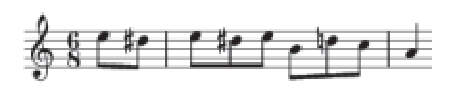
\includegraphics[scale=0.5]{figures/furelise.pdf}
%\end{minipage}
%\end{frame}
\end{document}
